\documentclass[journal]{IEEEtran}

\usepackage[T1]{fontenc}
\usepackage{amsmath,amssymb}
\usepackage{graphicx}
\usepackage{booktabs}
\usepackage{cite}
\usepackage[hidelinks]{hyperref}

\graphicspath{{figures/}}

\newcommand{\Rsq}{$R^2$}

\begin{document}

\title{What Transfers Across Studies? A Study-Grouped Audit of Machine Learning for Global Marine Microplastic Concentrations}

\author{Arnab~Chakraborty and Gourab~Adhikari%
\thanks{The authors are with the Department of Information Technology, Gauhati University, Guwahati, Assam, India.}%
\thanks{Manuscript draft, November 2026.}}

\markboth{Manuscript draft}{Chakraborty and Adhikari: A Study-Grouped Audit of Marine Microplastic Models}

\maketitle

\begin{abstract}
Machine learning studies of the NOAA NCEI Marine Microplastics database often report high accuracy under random cross-validation, but random splits put samples from the same cruise in both training and test sets. We audit what transfers to unseen studies using 16,988 ocean-water samples from 72 studies and 49 organizations, scoring every model over ten study-grouped fold assignments. Study identity explains 63.1\% of the variance in $\log_{10}$ concentration. LightGBM scores \Rsq{}~=~0.763 on random folds and 0.456 on unseen studies. Location and time alone score $-0.022$ on unseen studies. Sampling protocol (mesh size, depth, and sampler family) carries almost all of the transferable signal, much of it from two bulk-water studies whose archived concentrations are $10^6$ too small. Shallow trees raise unseen-study \Rsq{} to 0.527, and a Huber loss with a monotonic mesh constraint raises it to 0.543 and halves errors larger than a factor of 100 relative to the baseline. Weighted equally per study, the error improves much less (mean absolute error 1.04 to 1.02 in $\log_{10}$ units). A within-study drift-accumulation term adds 0.009 to pooled \Rsq{}. A two-part model that predicts detection and level separately gives the best held-out likelihood and reaches \Rsq{}~=~0.815 on detected samples. Study-grouped conformalized quantile regression covers 90.9\% of unseen-study samples at a nominal 90\%, where ensemble spread covers 15.2\%. The gains from the constraints vanish when the two corrected studies and one unverified study are removed.
\end{abstract}

\begin{IEEEkeywords}
Censored regression, conformal prediction, cross-validation, distribution shift, gradient boosting, marine microplastics, sampling protocol.
\end{IEEEkeywords}

\section{Introduction}

\IEEEPARstart{G}{lobal} compilations of marine microplastic measurements pool decades of shipboard surveys from dozens of research groups. The largest public compilation, the NOAA National Centers for Environmental Information (NCEI) Marine Microplastics database~\cite{ncei}, holds surveys that differ in sampler, mesh size, sampled volume, and laboratory protocol. A manta net with a 0.333~mm mesh typically reports 0.01 to 1 pieces/m$^3$. A Niskin bottle filtered through a membrane of a few micrometers reports 100 to 10,000 pieces/m$^3$, because particle counts rise steeply as the size cutoff falls~\cite{lindeque2020,tokai2021}. A single concentration column therefore mixes measurements that are not on the same physical scale.

Recent studies train gradient-boosted trees and learned representations on these compilations to map ocean microplastic concentrations~\cite{yu2023,amora2025,ali2026,chan2026,dalvi2026,narayanan2026}. Most report random $k$-fold scores. On NCEI data, a random split places neighboring stations from the same cruise on both sides of the split, so a model can score well by recognizing the cruise rather than by predicting a new one. Dalvi~\textit{et al.}~\cite{dalvi2026} documented a related failure across basins. Their XGBoost model reached \Rsq{}~=~0.651 on random folds and fell to between $-0.708$ and 0.166 when a whole ocean basin was held out. Uncertainty estimates share the weakness. Spread across an ensemble of seeds measures model variance, not the shift from one survey to the next, and its coverage on new surveys has not been tested.

This paper asks what a model trained on NCEI data can predict about a survey it has never seen, and how to make those predictions more accurate and more honest. We make six contributions.
\begin{enumerate}
\item We measure the gap between random and study-grouped validation on 16,988 samples from 72 studies. Every study-grouped score is a mean over ten study-fold assignments, alongside organization-grouped, chronological, and strict leave-one-ocean-out splits.
\item Through feature ablation we show that location and time transfer nothing to unseen studies, and that sampling protocol carries the transferable signal. We also show how much of that signal depends on two bulk-water studies.
\item We decompose the error of a standard gradient-boosted model and ablate three constraints that reduce it: shallow trees, a Huber loss, and a monotonic mesh constraint.
\item We test a within-study Lagrangian transport term and two censored models for non-detects, scored with a likelihood that is comparable across models.
\item We show that ensemble-spread intervals cover fewer than one in five unseen-study samples, and that study-grouped conformalized quantile regression (CQR)~\cite{romano2019} restores nominal coverage.
\item We document a $10^6$ unit error in two NCEI studies, verified against the primary publications, and report how every result changes without them.
\end{enumerate}

\section{Related Work}

\subsection{Machine Learning for Ocean Microplastic Concentration}

Yu~\textit{et al.}~\cite{yu2023} classified 1,169 global surface samples with random forest, GBDT, and XGBoost using 16 environmental and socio-economic predictors, reaching 0.719 accuracy and 0.914 ROC AUC on a random split. Amora~\cite{amora2025} reported \Rsq{}~=~0.972 on random splits using engineered regional concentration features. Narayanan~\cite{narayanan2026} classified about 20,000 NCEI records into five concentration tiers using coordinates, month, and SatCLIP geo-embeddings, and found inconsistent transfer across basins. Hafiz~\textit{et al.}~\cite{hafiz2026} linked MODIS reflectance to NCEI labels. Their models trained on the Bay of Bengal and East China Sea scored \Rsq{} between $-0.35$ and $-0.04$ on the Mediterranean.

The closest work is Dalvi~\textit{et al.}~\cite{dalvi2026}, who combined contrastive representation learning with XGBoost on NCEI data plus Copernicus and GEBCO predictors. On a $\ln(c+1)$ target with random five-fold validation they report \Rsq{}~=~0.651 and MAE~=~0.619. Leaving out one ocean, \Rsq{} is 0.166 (Indian), 0.082 (Pacific), 0.010 (Atlantic), $-0.253$ (Arctic), and $-0.708$ (Southern). They quantify uncertainty as $\hat{y}\pm1.96\sigma$ over ten XGBoost runs without reporting empirical coverage.

Regional studies report lower errors on narrower targets. Ali~\textit{et al.}~\cite{ali2026} predicted raw abundance at 346 Indian Ocean points (range 0 to 3.375, standard deviation 0.683) with \Rsq{}~=~0.861 and 93.3\% coverage at a nominal 90\% on a regional holdout. Chan~\textit{et al.}~\cite{chan2026} fused AOMI observations~\cite{isobe2021} with ERA5 and Argo data in the West Pacific for 2018 to 2020 and reported log-scale \Rsq{} of 0.64 to 0.88. Neither tests transfer across studies or sampling protocols.

\subsection{Study-Level Leakage, Harmonization, and Censoring}

Leakage across studies has been measured in related microplastic problems. Khanam~\textit{et al.}~\cite{khanam2026} found FTIR polymer classification macro-F1 falling from 0.972 on random splits to 0.672 when whole studies were held out. Monreal Hern\'andez~\cite{monreal2026} reported a similar collapse for adsorption models, and Mokeira~\textit{et al.}~\cite{mokeira2026} quantified geographic confounding in global soil microplastic prediction. Meyer and Pebesma~\cite{meyer2021} proposed restricting spatial models to their area of applicability, which motivates the out-of-support flags in Section~\ref{sec:flags}.

Koelmans~\textit{et al.}~\cite{koelmans2020} proposed rescaling counts between size windows with a power law. The rescaling requires the lower and upper size limits of each measurement plus a compartment-specific exponent. NCEI does not record both limits consistently, so we model protocol directly instead. Three ideas from outside machine learning shape our fixes. Maximenko~\textit{et al.}~\cite{maximenko2012} showed that drifter-derived surface currents gather floating debris in subtropical convergence zones, where currents are slow. Helsel~\cite{helsel2012} argued that environmental zeros are non-detects below a detection limit and should be modeled as censored. Mundlak~\cite{mundlak1978} separated within-cluster slopes from between-cluster confounding in panel data.

\section{Data}

\subsection{Source and Filtering}

We use the NCEI Marine Microplastics export~\cite{ncei}, which holds 29,076 records in 35 columns. The concentration column mixes pieces/m$^3$ for water and beach sand, pieces/kg for sediment, and Nurdle Patrol counts. Keeping rows with marine setting ``Ocean water'' and unit pieces/m$^3$ leaves 16,988 samples collected from 1972 to 2024, from 73 NCEI accessions and 73 DOIs. The organization field lists the Galway-Mayo Institute of Technology under three names, including its successor, Atlantic Technological University, and Italy's National Research Council under two. Merging these reduces 52 organization names to 49.

\subsection{Unit Errors}

Two studies in the export are too small by a factor of $10^6$. In both, a concentration in pieces/L appears to have been divided by 1,000 rather than multiplied when converted to pieces/m$^3$.
\begin{itemize}
\item Barrows~\textit{et al.}~\cite{barrows2018} (1,389 grab samples). The preprint reports a mean of 11.8 particles/L, or 11,800 pieces/m$^3$. NCEI stores a mean of 0.0128 pieces/m$^3$.
\item Dehm~\textit{et al.}~\cite{dehm2020} (81 Niskin samples). The abstract reports 1.6 to 2.0 particles/L. NCEI stores a mean of 0.00176 pieces/m$^3$.
\end{itemize}
We multiply both studies by $10^6$ and repeat the main analyses with both removed. NCEI has not yet corrected the archive. A third study, 33 bongo-net samples from Arteaga~\textit{et al.}~\cite{arteaga2024}, has a median of 2,860 pieces/m$^3$, which is high for a net. Its abstract mixes units and its full text is paywalled, so we leave it unchanged and test its removal separately.

Barrows~\textit{et al.} count all microparticles. Of 113 particles they checked by FTIR, 57\% were synthetic, 12\% semi-synthetic, and 31\% natural. This study therefore measures a broader quantity than most net surveys.

\subsection{Target and Study Definition}

Concentrations span eight orders of magnitude, and 64\% lie below 0.1 pieces/m$^3$, where $\ln(c+1)$ is almost the identity. We model
\begin{equation}
y=\log_{10}(c+10^{-3}),
\end{equation}
where $c$ is concentration in pieces/m$^3$. The offset is close to the smallest non-zero surface-net value ($6.8\times10^{-4}$) and maps zeros to $-3$. An absolute error of 1 on this scale is a factor of ten.

We define a study as a connected component of records that share a DOI or an NCEI accession, which gives 72 studies. The largest, from the Sea Education Association (1986 to 2008), holds 6,135 samples, or 36\% of the data. Fourteen organizations contributed more than one study, so we also group by organization.

\section{Methods}

\subsection{Features and Baseline Models}

Baseline models use seven numeric features (latitude, longitude, year, $\sin$ and $\cos$ of month, $\log_{10}$ mesh size, and $\ln(1+\text{depth})$) and one categorical feature, the sampler family. The 17 lowercased method strings map to three families. Neuston, manta, plankton, AVANI, and bongo nets form the surface-net family, the three pump methods form the pump family, and the nine bottle, bucket, jar, rosette, and grab methods form the bulk-water family. Missing depths (0.3\%) take the training-fold median, except in CatBoost, which handles missing values itself. Numeric features enter tree models unscaled. We call mesh size, depth, and family the \emph{protocol} features.

We compare eight baselines. The study-mean predictor returns the training mean of the sample's study, or the global mean for an unseen study. Linear regression uses features clipped to the training range, and $k$-nearest neighbors averages the 15 nearest samples by haversine distance, weighted by inverse distance. The tree models are random forest~\cite{breiman2001} with 300 trees and at least 3 samples per leaf, XGBoost~\cite{chen2016} with 500 trees of depth 6, LightGBM~\cite{ke2017} with 500 trees, and CatBoost~\cite{prokhorenkova2018} with 500 iterations and the method string as an extra categorical feature. An XGBoost hurdle model mixes a detection classifier with a regressor on positive samples. All boosters use a learning rate of 0.05.

\subsection{Validation Schemes}

\begin{enumerate}
\item \emph{Random}: five folds over samples.
\item \emph{Study-grouped}: five folds over studies, repeated over ten random assignments of studies to folds (seeds 0 to 9). We report the mean over the ten assignments, because a single assignment can move \Rsq{} by more than 0.15.
\item \emph{Organization-grouped}: five folds over the 49 organizations, so a second cruise by the same group cannot sit in training. We repeat it over ten assignments in the same way.
\item \emph{Chronological}: train before 2015 and test on 2015 onward (4,638 samples), with test studies split into those seen and unseen in training.
\item \emph{Strict leave-one-ocean-out (LOOO)}: hold out each of the Indian, Pacific, Atlantic, Arctic, and Southern basins, and drop from training any study that also sampled the held-out basin.
\end{enumerate}

\subsection{Metrics and Study-Constant Oracle}

On the $y$ scale we report pooled \Rsq{}, MAE, the share of samples within a factor of ten ($|\hat{y}-y|\le1$), and the share of errors larger than a factor of 100 ($|\hat{y}-y|>2$). Because the largest study holds 36\% of the samples, we also report \emph{study MAE}, the mean over studies of each study's MAE, which weights every study equally. As a reference we report a \emph{study-constant oracle}. It is told each unseen study's true level and predicts it for every sample in that study. Its \Rsq{} uses the study mean (0.666), and its MAE and threshold metrics use the study median (MAE 0.708, a factor of 5.1). The oracle has perfect between-study skill and no within-study skill. A model that predicts variation inside studies could in principle beat it.

\subsection{Environmental Covariates}

To test whether place descriptors transfer better than raw coordinates, we compute six covariates from each sample's location and month. Natural Earth~\cite{naturalearth} gives the distance to the nearest coast and the population within 200~km. Meijer~\textit{et al.}~\cite{meijer2021} give the distance to the nearest of the 1,000 largest river plastic outlets and the summed modeled emission of all outlets within 200~km. The 1991--2020 NOAA OISST climatology~\cite{reynolds2002} gives monthly sea surface temperature, and the Global Drifter Program climatology~\cite{laurindo2017} gives current speed. We fixed the radii and the outlet count before running any model. We add the six covariates to LightGBM and to CatBoost without the method string, over the same ten assignments.

\subsection{Few-Sample Calibration and Within-Study Ranking}

A new survey could measure a few samples first and use them to correct the model. For each held-out study we reveal $k$ of its samples, drawn at random from a pool of up to 20 samples and at most half the study. We shift every prediction for that study by the summed error on the revealed samples divided by $k+\lambda$, where $\lambda=(1-\text{ICC})/\text{ICC}$ is the usual shrinkage for a random intercept, with the ICC estimated on the training studies of each fold. Scores use only samples outside the pool, so every $k$ is scored on the same samples. The reference is the global training mean, calibrated the same way. To test whether models rank samples within a study, we compute the Spearman correlation between prediction and truth inside each of the 50 studies with at least 20 samples. A study with constant predictions counts as zero.

\subsection{Diagnosing the Baseline Error}

We split the out-of-fold squared error of baseline LightGBM on unseen studies into a between-study and a within-study part, averaged over the ten assignments. The mean squared error is 2.073. Two problems stand out.

\emph{Spurious within-study variance.} The true variance of $y$ around each study's mean is 1.274. LightGBM's within-study squared error is 1.504, which is 72.5\% of its total error and 0.230 more than predicting a constant for each study would give. Unconstrained interactions between coordinates, year, and protocol make predictions vary inside a study (variance 0.359) while barely tracking the true order of stations (correlation 0.096).

\emph{A cliff at zero.} One particle in a one-liter sample is 1,000 pieces/m$^3$, or $y=3$. Coding an empty one-liter bottle as $y=-3$ places it six orders of magnitude below the smallest value the method can detect. In the bulk-water family 19.2\% of samples are zeros, from Barrows~\textit{et al.}, McEachern~\textit{et al.}~\cite{mceachern2019}, Dehm~\textit{et al.}, and Kanhai~\textit{et al.}~\cite{kanhai2018}. Barrows~\textit{et al.} alone produce 37.2\% of the squared error over the whole dataset. Across the 11 bulk-water studies with at least five samples, the Pearson correlation between study-mean $\log_{10}$ mesh size and study-mean $y$ is $-0.732$ on positive samples and $+0.228$ on all samples. The zeros reverse the sign of the mesh effect.

\subsection{Constrained Protocol Trees}

The first fix limits what the trees can learn. The constrained model is LightGBM on the protocol features with depth 3, 7 leaves, 150 trees, and at least 30 samples per leaf. It adds a Huber loss (LightGBM's default threshold of 0.9) to bound the influence of the zero cliff. It also adds a decreasing monotonic constraint on $\log_{10}$ mesh size, since finer meshes retain more particles~\cite{lindeque2020,tokai2021}. We ablate the three parts. A separate variant keeps all features and forbids interactions between the protocol group and a space-time group (latitude, longitude, year, and month). It uses 200 trees and at least 50 samples per leaf, with the same depth, leaf limit, Huber loss, and mesh constraint.

\subsection{Within-Between Lagrangian Transport}

Floating debris collects where surface currents converge~\cite{maximenko2012}. To turn this into a feature with no fitted parameters, we take the 1$^\circ$ annual-mean Global Drifter Program velocity climatology~\cite{laurindo2017} and release 80,000 passive tracers uniformly over ocean cells. We advect them for five years in 5-day steps with a small random walk (0.15 grid cells per step) and reject moves onto land. The final tracer density, smoothed with a 2.5-cell Gaussian kernel, gives $a=\ln(1+\text{density})$. Each sample takes the value of its nearest ocean cell by haversine distance.

Fitted directly to $y$, any place-based feature can act as a proxy for which cruise sampled there. We therefore estimate its effect only from variation inside studies. For surface-net samples $i$ in training study $s$, let $\tilde{a}_i=a_i-\bar{a}_s$ and $\tilde{y}_i=y_i-\bar{y}_s$, with means taken over the study's surface-net samples. We fit
\begin{equation}
\beta=\max\!\left(0,\;\frac{\sum_i\tilde{a}_i\tilde{y}_i}{\sum_i\tilde{a}_i^2}\right)
\end{equation}
inside each training fold. Because $\tilde{a}$ and $\tilde{y}$ have zero mean in every study, $\beta$ cannot absorb differences between studies. Across the 50 training folds, $\beta$ ranges from 0.049 to 0.354 (median 0.208). We subtract $\beta a$ from the training target of surface-net samples, fit the constrained protocol tree to the adjusted target, and add $\beta a$ back to surface-net test predictions. We call this model \emph{Within-Between Physics}. A variant adds a second-stage tree on coordinates and month, fitted to within-study residuals, with its weight chosen from $\{0, 0.25, 0.5, 0.75, 1\}$ by inner study-grouped cross-validation.

\subsection{Left-Censored Models}

The second fix treats a zero as below the detection limit rather than as $10^{-3}$. Inside each training fold, we set the detection limit $L$ on the $\log_{10}$ scale for each combination of sampler family and mesh class (below 0.05~mm, or 0.05~mm and above). It is the $\log_{10}$ of the median, across studies, of each study's smallest positive concentration. Let $z=\log_{10}c$ for positive samples. We compare three models.
\begin{itemize}
\item The \emph{baseline} keeps zeros at $y=-3$. Its regression gives the level of positive samples, and a separate LightGBM classifier on all features gives $P(c>0)$. Both classifiers in this section use 150 trees of depth 3 with at least 30 samples per leaf.
\item A \emph{two-part} model uses a LightGBM detection classifier on the protocol features and a level model trained on positive samples only. The level model is either the constrained protocol tree or Within-Between Physics.
\item A \emph{left-censored (Tobit) LightGBM} on the protocol features, with the Within-Between transport offset, minimizes
\begin{equation}
\ell_i=\begin{cases}\dfrac{(f_i-z_i)^2}{2\sigma^2}+\ln\sigma+\tfrac{1}{2}\ln 2\pi, & c_i>0,\\[2mm] -\ln\Phi\!\left(\dfrac{L_i-f_i}{\sigma}\right), & c_i=0,\end{cases}
\end{equation}
which is convex in $f_i$. We boost with its exact gradient and Hessian at $\sigma=0.9$. Its detection probability is $1-\Phi((L-f)/\sigma)$, and its level for a detected sample is the truncated-normal mean $f+\sigma\lambda((f-L)/\sigma)$, where $\lambda$ is the inverse Mills ratio.
\end{itemize}
We cannot score the models with $\ell_i$. The detection limit is a median of per-study minimums, not a hard floor, and 32\% to 39\% of detected test samples lie below it, depending on the assignment. A Tobit model assigns those samples no probability. All models are therefore scored with the same held-out mixed likelihood. A zero costs $-\ln(1-p)$, and a positive sample costs $-\ln p$ plus a Gaussian negative log-likelihood of $z$ around the model's predicted level, where $p$ is the model's detection probability. We also report the two parts separately. The level spread $\sigma_z$ is the root-mean-square residual of inner study-grouped out-of-fold level predictions on positive training samples. For the Tobit model, the $\sigma$ inside its detection probability and truncated mean is the grid value from 0.3 to 2.5 that minimizes the same mixed likelihood on those inner out-of-fold predictions.

\subsection{Prediction Intervals and Reliability Flags}
\label{sec:flags}

Within each outer study-grouped fold we build 90\% intervals in four ways.
\begin{enumerate}
\item \emph{Ensemble spread}: ten LightGBM models with varied seeds, depths, and subsampling give $\hat{y}\pm1.645\sigma$ (and $\pm1.96\sigma$ for 95\%), following~\cite{dalvi2026}.
\item \emph{Random-CV conformal}: symmetric split-conformal intervals calibrated on five random inner folds.
\item \emph{Study-grouped conformal}: symmetric intervals calibrated on four study-grouped inner folds, with either equal weight per sample (row) or weight inversely proportional to study size (study).
\item \emph{Study-grouped CQR}~\cite{romano2019}: LightGBM quantile models at 0.05 and 0.95 on all features, with conformity scores $\max(\hat{q}_{lo}-y,\,y-\hat{q}_{hi})$ calibrated on the same inner folds, with row or study weights.
\end{enumerate}

We also compute binary label-free flags from each training fold: a method string not seen in training, a bulk-water or pump sampler, a mesh outside the training range, a distance over 500~km to any training sample, a distance over 500~km to any training sample of the same family, and membership in the widest quarter of study-weighted CQR intervals, ranked across all out-of-fold predictions in an assignment. For selective prediction, we rank test samples by one of four continuous risk scores (CQR interval width, ensemble standard deviation, distance to the nearest same-family training sample, and the count of the first, second, third, and fifth flags) and measure error on the samples kept as the riskiest are deferred.

\section{Results}

\subsection{Random Splits Overstate Transfer}

A random-intercept model $y\sim1+(1\,|\,\text{study})$ gives an intraclass correlation of 0.631, so almost two-thirds of the variance in $y$ lies between studies. Table~\ref{tab:baseline} shows the consequence. On random folds the tree ensembles reach \Rsq{} of 0.748 to 0.767. Predicting each sample's training-study mean already scores 0.664 on random folds and $-0.288$ on unseen studies, so much of a random-split score comes from recognizing the study. On unseen studies the best models are CatBoost (0.481) and LightGBM (0.456), and spatial $k$NN falls to $-1.973$.

Pooled \Rsq{} also hides how uneven the folds are. The Sea Education Association study holds 36\% of the samples, so the fold that contains it dominates the pooled score. Averaged per fold instead of pooled, LightGBM scores 0.118 and CatBoost 0.252, and most other models score near zero. On the chronological split, random forest is the only baseline above zero on test studies unseen in training (0.122).

\begin{table*}[!t]
\centering
\caption{Baseline models. Study-grouped columns are means over ten study-grouped fold assignments. Fold \Rsq{} averages per-fold scores instead of pooling them. The chronological columns use one train-before-2015 split, scored on all test samples and on test studies unseen in training. Bold marks the best value in each column.}
\label{tab:baseline}
\begin{tabular}{@{}lcccccccc@{}}
\toprule
 & Random & \multicolumn{5}{c}{Study-grouped} & \multicolumn{2}{c}{Chronological \Rsq}\\
\cmidrule(lr){3-7}\cmidrule(lr){8-9}
Model & \Rsq & \Rsq & Fold \Rsq & MAE & Study MAE & Within $10\times$ & All & Unseen studies\\
\midrule
Study mean only & 0.664 & $-0.288$ & $-0.825$ & 1.790 & 1.548 & 28.0\% & $-0.228$ & $-0.958$\\
Linear regression & 0.545 & 0.394 & 0.025 & 1.163 & 1.125 & 52.4\% & $-1.668$ & $-4.665$\\
Spatial $k$NN & 0.560 & $-1.973$ & $-3.414$ & 2.790 & 1.422 & 24.1\% & $-0.489$ & $-0.904$\\
Random forest & 0.764 & 0.428 & 0.024 & 1.052 & 1.099 & \textbf{64.5\%} & \textbf{0.257} & \textbf{0.122}\\
XGBoost & 0.757 & 0.347 & $-0.004$ & 1.102 & 1.127 & 62.7\% & 0.196 & $-0.036$\\
LightGBM & 0.763 & 0.456 & 0.118 & 1.048 & 1.041 & 62.0\% & 0.110 & $-0.231$\\
CatBoost & 0.748 & \textbf{0.481} & \textbf{0.252} & \textbf{1.009} & \textbf{0.979} & \textbf{64.5\%} & 0.165 & $-0.137$\\
XGBoost hurdle & \textbf{0.767} & 0.399 & 0.030 & 1.073 & 1.084 & 61.8\% & 0.078 & $-0.278$\\
\bottomrule
\end{tabular}
\end{table*}

For a scale-matched reference, the same LightGBM on the $\ln(c+1)$ target of Dalvi~\textit{et al.} scores \Rsq{}~=~0.815 and MAE~=~0.368 on random folds, against their reported 0.651 and 0.619. With location and time alone it still scores 0.786. The feature sets and data versions differ, so this shows that a high random-split score is easy to reach on this data, not that our model is better.

\subsection{Protocol Carries the Transferable Signal}

Table~\ref{tab:sensitivity} separates the feature groups. On the full data, LightGBM with location and time alone scores 0.741 on random folds and $-0.022$ on unseen studies. Protocol features alone score 0.428, close to all features together (0.456). Location and time therefore add almost nothing that transfers, and protocol carries nearly all of what does.

The environmental covariates point the same way. Adding the six place descriptors lowers mean grouped \Rsq{} from 0.456 to 0.449 for LightGBM (better in 5 of 10 assignments) and from 0.453 to 0.428 for CatBoost (3 of 10). On their own the descriptors score $-1.024$ and $-0.967$. Six continuous descriptors of a place identify it about as precisely as its coordinates do, so the trees use them to recognize a study's region.

Calibration and ranking place the models' skill. With no revealed samples the models are far ahead of the global mean ($-0.305$), with LightGBM at 0.457 and Within-Between Physics at 0.557. Three revealed samples lift the calibrated global mean to 0.556, above calibrated LightGBM in all ten assignments and above calibrated CatBoost in five. The constrained protocol and Within-Between Physics models stay ahead of it through five samples (0.600 and 0.596 against 0.595, better in 8 and 6 of 10 assignments). They trail slightly at ten samples (0.617 and 0.616 against 0.624) and at twenty (0.640 and 0.641 against 0.647). Inside the 50 unseen studies with at least 20 samples, the median Spearman correlation between prediction and truth is 0.059 for LightGBM and 0.025 for CatBoost. The constrained protocol model gives the same prediction to almost every sample of a study, so its median is zero and only 6.2\% of studies are positive. Within-Between Physics varies mainly inside surface-net studies, through the drift term. Its median over all 50 studies is also zero, but 43.6\% are positive (Section~\ref{sec:drift}). Shifting each model's predictions to the true study mean gives \Rsq{} of 0.606 (LightGBM) to 0.660 (Within-Between Physics), all below the 0.666 of the true study mean alone. The models estimate a study's level, mostly from its protocol, and their variation within a study only adds error.

\subsection{Sensitivity to Disputed Studies}

Table~\ref{tab:sensitivity} also repeats the audit without the unit-corrected and unverified studies. The gap between random and study-grouped validation holds in every subset (0.761 to 0.768 against 0.223 to 0.467), and location and time stay near zero on unseen studies (at most 0.128). The advantage of protocol does not hold as well. Without Barrows and Dehm, protocol alone falls to 0.100, against 0.055 for location and time. These two studies supply the only fine-mesh bulk-water samples in large numbers, and much of what protocol transfers is the difference between bulk water and nets. Removing the 33 bongo-net samples raises grouped \Rsq{} slightly, so they do not inflate the result.

\begin{table}[!t]
\centering
\caption{LightGBM audit with disputed studies removed. Grouped columns are means over ten study-grouped fold assignments. B\&D: Barrows and Dehm. Bongo: Arteaga~\textit{et al.}}
\label{tab:sensitivity}
\setlength{\tabcolsep}{3pt}
\begin{tabular}{@{}lcccccc@{}}
\toprule
 & & & Random & \multicolumn{3}{c}{Study-grouped \Rsq}\\
\cmidrule(lr){5-7}
Subset & Studies & ICC & \Rsq & All & Protocol & Loc.+time\\
\midrule
Full data & 72 & 0.631 & 0.763 & 0.456 & 0.428 & $-0.022$\\
Without bongo & 71 & 0.612 & 0.761 & 0.467 & 0.490 & 0.009\\
Without B\&D & 70 & 0.739 & 0.768 & 0.223 & 0.100 & 0.055\\
Without all three & 69 & 0.720 & 0.766 & 0.397 & 0.263 & 0.128\\
\bottomrule
\end{tabular}
\end{table}

\subsection{Which Constraints Help}

Table~\ref{tab:ablation} ablates the constrained protocol model over the ten assignments. Shallow trees alone raise mean \Rsq{} from 0.428 (deep protocol trees) to 0.527, which is most of the gain. Adding the Huber loss and the monotonic mesh constraint together raises \Rsq{} to 0.543 (better than shallow trees alone in 6 of 10 assignments), lowers MAE from 0.993 to 0.931, and cuts errors above a factor of 100 from 10.0\% to 7.1\%. Per study the picture differs. Shallow trees alone cut study MAE from 1.281 (deep protocol trees) to 1.096, still worse than the all-feature baseline (1.041). Adding the Huber loss brings it to 1.038, and the full constrained model reaches 1.021. Neither addition helps on its own in every metric. The Huber loss alone lowers \Rsq{} (0.512), and the monotonic constraint alone lowers the LOOO mean (0.313). Shallow trees with squared loss have the best LOOO mean (0.405), and shallow trees with the monotonic constraint have the best organization-grouped \Rsq{} (0.373).

\begin{table}[!t]
\centering
\caption{Ablation of the constrained protocol model. \Rsq{}, MAE, St.\ MAE, and errors above $100\times$ are means over ten study-grouped fold assignments, Org.\ \Rsq{} is the mean over ten organization-grouped assignments, and LOOO is the strict leave-one-ocean-out mean. St.\ MAE is study MAE, which weights every study equally. Shal.: shallow trees. Hub.: Huber loss. Mono.: monotonic mesh constraint. Bold marks the best value in each column.}
\label{tab:ablation}
\setlength{\tabcolsep}{3pt}
\begin{tabular}{@{}ccccccccc@{}}
\toprule
Shal. & Hub. & Mono. & \Rsq & MAE & St.\ MAE & $>100\times$ & Org.\ \Rsq & LOOO\\
\midrule
 & & & 0.428 & 1.073 & 1.281 & 13.3\% & 0.218 & 0.360\\
\checkmark & & & 0.527 & 0.993 & 1.096 & 10.0\% & 0.334 & \textbf{0.405}\\
\checkmark & \checkmark & & 0.512 & 0.967 & 1.038 & 8.5\% & 0.305 & 0.379\\
\checkmark & & \checkmark & 0.534 & 0.980 & 1.086 & 9.3\% & \textbf{0.373} & 0.313\\
\checkmark & \checkmark & \checkmark & \textbf{0.543} & \textbf{0.931} & \textbf{1.021} & \textbf{7.1\%} & 0.367 & 0.385\\
\bottomrule
\end{tabular}
\end{table}

\subsection{Constrained and Within-Between Models}

Table~\ref{tab:v2} and Fig.~\ref{fig:benchmark} compare the main models. The constrained protocol model beats the baseline in 9 of 10 assignments. Adding the within-study drifter term raises \Rsq{} to 0.552. It beats the baseline in all ten assignments, and its worst assignment (0.476) is above the baseline mean. Against the constrained protocol model the gain is only 0.009, and it wins 7 of 10 assignments. Of the 0.096 total gain over the baseline, the constrained protocol model supplies 0.087. A second-stage coordinate tree adds nothing (0.550), so raw coordinates hold no within-study signal that transfers.

Weighting studies equally shrinks these gains. The constrained protocol model and Within-Between Physics lower study MAE only from 1.041 to 1.021 and 1.020, and the interaction-constrained model (0.978) and CatBoost (0.979, Table~\ref{tab:baseline}) do better. Much of the pooled gain therefore comes from the largest studies, where the constraints remove spurious variation across thousands of samples.

On the other validation schemes the ranking changes. Among the models in Table~\ref{tab:v2}, the interaction-constrained model has the highest organization-grouped \Rsq{} (0.407) and LOOO mean (0.432). It is also the only LightGBM variant above zero on post-2015 studies unseen in training (0.011, against $-0.071$ for Within-Between Physics and $-0.231$ for the baseline). Grouping by organization lowers every model by 0.09 to 0.21 against grouping by study (the baseline falls from 0.456 to 0.282). No model predicts future surveys well, and the best model depends on the kind of transfer asked for.

\begin{table*}[!t]
\centering
\caption{Main models over ten study-grouped fold assignments, ten organization-grouped fold assignments (49 organizations), and strict leave-one-ocean-out. Wins count the study-grouped assignments in which a model beats baseline LightGBM. Bold marks the best value in each column, excluding the oracle.}
\label{tab:v2}
\setlength{\tabcolsep}{3pt}
\begin{tabular}{@{}lccccccccc@{}}
\toprule
Model & \Rsq{} mean & Range & Wins & MAE & Study MAE & Within $10\times$ & $>100\times$ & Org.\ \Rsq & LOOO mean (min)\\
\midrule
Baseline LightGBM, all features & 0.456 & 0.388--0.545 & -- & 1.048 & 1.041 & 62.0\% & 14.2\% & 0.282 & 0.208 ($-0.146$)\\
LightGBM, protocol only & 0.428 & 0.263--0.525 & 4/10 & 1.073 & 1.281 & 63.8\% & 13.3\% & 0.218 & 0.360 (0.100)\\
LightGBM, location and time only & $-0.022$ & $-0.083$--0.099 & 0/10 & 1.444 & 1.399 & 49.4\% & 24.6\% & $-0.117$ & $-0.333$ ($-0.788$)\\
Constrained protocol & 0.543 & 0.433--0.567 & 9/10 & 0.931 & 1.021 & \textbf{68.3\%} & \textbf{7.1\%} & 0.367 & 0.385 (0.078)\\
Interaction-constrained & 0.511 & 0.449--0.559 & 9/10 & 0.976 & \textbf{0.978} & 62.2\% & 8.7\% & \textbf{0.407} & \textbf{0.432} (0.126)\\
Constrained protocol + coordinate stage & 0.543 & 0.435--0.562 & 9/10 & 0.931 & 1.014 & 67.7\% & 7.6\% & 0.370 & 0.396 (0.113)\\
Within-Between Physics & \textbf{0.552} & 0.476--0.575 & \textbf{10/10} & \textbf{0.929} & 1.020 & 65.8\% & 7.4\% & 0.373 & 0.418 (0.194)\\
Within-Between Physics + coordinate stage & 0.550 & 0.467--0.570 & \textbf{10/10} & 0.931 & 1.014 & 65.9\% & 7.6\% & 0.362 & 0.418 (\textbf{0.203})\\
\midrule
Study-constant oracle (reference) & 0.666 & -- & -- & 0.708 & 0.519 & 81.5\% & 5.6\% & -- & --\\
\bottomrule
\end{tabular}
\end{table*}

\begin{figure*}[!t]
\centering
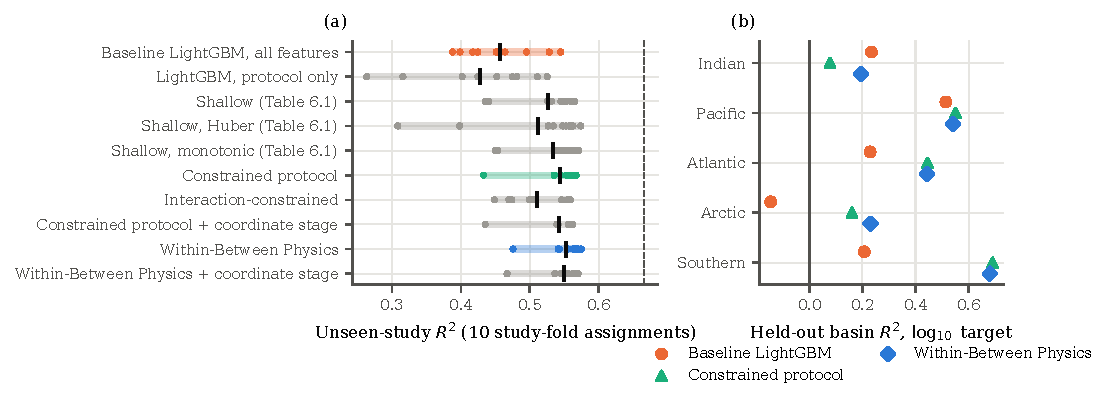
\includegraphics[width=\textwidth]{fig_benchmark.pdf}
\caption{(a) Pooled \Rsq{} on unseen studies for each of ten study-fold assignments (dots), their range (bar), and mean (vertical tick), for the models in Tables~\ref{tab:ablation} and~\ref{tab:v2} except location and time only. The dashed line is the study-constant oracle. (b) \Rsq{} on each held-out basin under strict leave-one-ocean-out on the $\log_{10}$ target.}
\label{fig:benchmark}
\end{figure*}

\subsection{Leave-One-Ocean-Out}

On the $\log_{10}$ target (Fig.~\ref{fig:benchmark}b), adding coordinates and time to protocol features hurts in four of five basins. The Atlantic drops from 0.547 with protocol alone to 0.229 with all features. Within-Between Physics is positive in every basin (Indian 0.194, Pacific 0.541, Atlantic 0.444, Arctic 0.231, Southern 0.680). Against the constrained protocol model, the drifter term mainly helps the Indian (0.078 to 0.194) and Arctic (0.161 to 0.231) basins and changes the other three by 0.011 or less. The Southern Ocean holds only 27 samples from three studies, so its score is noisy.

These scores cannot be compared with those of Dalvi~\textit{et al.}, who used $\ln(c+1)$. We therefore refit the models on $\ln(c+1)$ (Fig.~\ref{fig:dalvi}). LightGBM with location and time alone reproduces their failure. It is negative in four of five basins and reaches $-3.00$ in the Indian Ocean. The protocol-only, constrained, and Within-Between models are positive in all five basins on this scale, while the all-features baseline still scores $-0.267$ in the Arctic. The constrained protocol model scores 0.564 to 0.704 (mean 0.648), above the values Dalvi~\textit{et al.} report in every basin. The drifter term adds nothing on this scale (mean 0.640). Four differences remain. We apply the unit correction, which places the median of the 1,470 corrected bulk-water samples at $\ln(c+1)=8.3$ while the surface-net median is 0.011, so part of our higher \Rsq{} comes from that larger, protocol-driven spread. Our strict study exclusion removes more training data than a plain basin split. Their model uses environmental predictors that ours does not. Their data version may differ from ours.

\begin{figure}[!t]
\centering
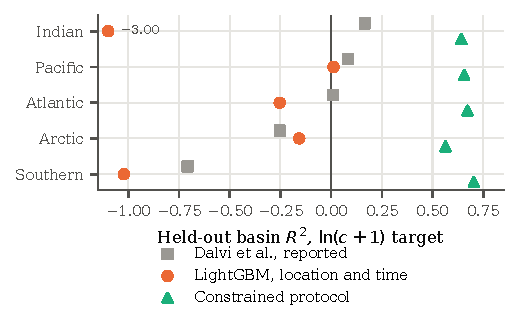
\includegraphics[width=\columnwidth]{fig_dalvi_scale.pdf}
\caption{Strict leave-one-ocean-out \Rsq{} on the $\ln(c+1)$ target of Dalvi~\textit{et al.}~\cite{dalvi2026}, against the values they report. The Indian Ocean value for location and time is clipped at the axis edge.}
\label{fig:dalvi}
\end{figure}

\subsection{Drift Accumulation Inside Surface-Net Studies}
\label{sec:drift}

The drifter term earns its place inside comparable surveys rather than in the global score. We take the 32 surface-net studies with at least 20 samples in which every candidate feature varies. In these studies the median within-study Spearman correlation between $a$ and $y$ is $+0.141$, positive in 62.5\% of studies. Scalar current speed from the same climatology correlates negatively ($-0.100$, positive in 34.4\%). Latitude ($+0.045$), absolute latitude (0.000), and longitude ($-0.038$) correlate near zero. Debris collects where currents are weak, as the convergence-zone picture predicts.

On the 14,233 surface-net samples from 58 studies (Fig.~\ref{fig:physics}a), baseline LightGBM scores a mean \Rsq{} of only 0.035 over ten assignments. The constrained protocol model reaches 0.253, and Within-Between Physics reaches 0.275 and beats it in all ten assignments. The oracle reaches 0.553. These gains are fragile. The worst assignment is negative for every model ($-0.170$ for Within-Between Physics), and every model scores below zero on the organization-grouped split of this subset. There the baseline ($-0.179$) does better than the constrained protocol model ($-0.289$) and Within-Between Physics ($-0.327$). Predicting a new organization's net survey from other organizations' net surveys remains unsolved.

\begin{figure*}[!t]
\centering
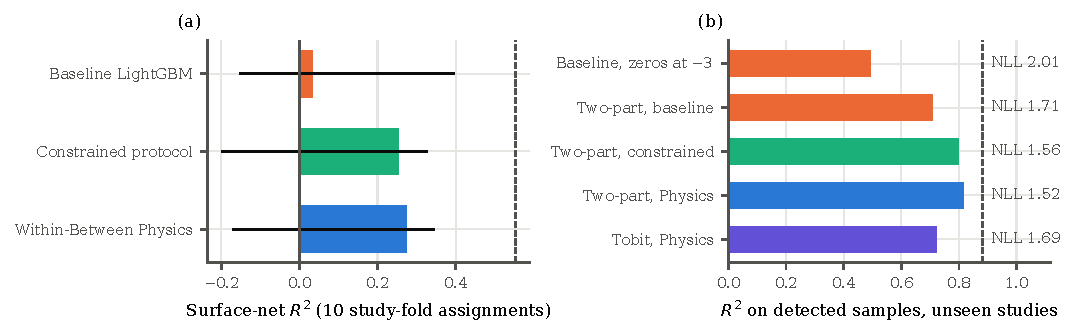
\includegraphics[width=\textwidth]{fig_surface_censored.pdf}
\caption{(a) Mean \Rsq{} on the surface-net subset over ten study-grouped fold assignments, with the range across assignments. (b) Unseen-study \Rsq{} on detected samples, with the held-out negative log-likelihood (NLL, lower is better) on all samples. Dashed lines are the study-constant oracle.}
\label{fig:physics}
\end{figure*}

\subsection{Non-Detects}

Table~\ref{tab:censored} and Fig.~\ref{fig:physics}b score the censored models. The two-part Within-Between Physics model gives the best held-out likelihood (NLL 1.519, against 1.691 for the Tobit model and 2.005 for the baseline). It also predicts the level of detected samples best, with \Rsq{}~=~0.815 and MAE~=~0.633 (a factor of 4.3). In that model 80.9\% of detected samples fall within a factor of ten and 1.3\% are off by more than 100. The oracle on detected samples reaches 0.882 and an MAE of 0.501. The Tobit model ranks detections best (AUC 0.700 against 0.630), because detection and level share one function. Its detection probabilities are worse calibrated, though (log-loss 0.697 against 0.642), and its level for detected samples is less accurate (\Rsq{}~=~0.723). Every model predicts zeros poorly. That points at sampled volume, which NCEI does not record consistently.

\begin{table}[!t]
\centering
\caption{Censored models over ten study-grouped fold assignments. NLL is the mixed likelihood on all samples, and Det.\ is its detection part (log-loss). \Rsq{}, MAE, and errors above $100\times$ are on detected samples only. Bold marks the best value in each column, excluding the oracle.}
\label{tab:censored}
\setlength{\tabcolsep}{2.5pt}
\begin{tabular}{@{}lcccccc@{}}
\toprule
Model & NLL & Det. & AUC & \Rsq{} & MAE & $>100\times$\\
\midrule
Baseline (zeros at $-3$) & 2.005 & 0.656 & 0.617 & 0.493 & 0.980 & 12.6\%\\
Two-part, constrained & 1.559 & \textbf{0.642} & 0.630 & 0.798 & 0.665 & 1.8\%\\
Two-part, Physics & \textbf{1.519} & \textbf{0.642} & 0.630 & \textbf{0.815} & \textbf{0.633} & \textbf{1.3\%}\\
Tobit, Physics & 1.691 & 0.697 & \textbf{0.700} & 0.723 & 0.805 & 2.7\%\\
\midrule
Study-constant oracle & -- & -- & -- & 0.882 & 0.501 & 1.1\%\\
\bottomrule
\end{tabular}
\end{table}

\subsection{Prediction Intervals}

Table~\ref{tab:intervals} and Fig.~\ref{fig:intervals} report intervals for baseline LightGBM on unseen studies, averaged over the ten assignments. Ensemble spread covers 15.2\% of samples at a nominal 90\% and 18.4\% at a nominal 95\%. It measures disagreement between models, not the shift to a new survey. Conformal intervals calibrated on random inner folds cover 71.2\%. Symmetric intervals calibrated across studies reach 87.1\% to 87.9\%, still short of 90\%. Study-grouped CQR reaches nominal coverage (90.6\% with row weights and 90.9\% with study weights). With study weights its median width is 3.85 $\log_{10}$ units, 24\% narrower than the row-weighted symmetric interval. A median width of 3.85 $\log_{10}$ units is a factor of 84 on either side of the interval's center, or a span of about 7,100 from bound to bound. That states plainly how little a new survey's protocol and location constrain its concentration.

Within-Between Physics point predictions narrow the row-weighted symmetric study-grouped interval from 5.09 to 4.31 $\log_{10}$ units and raise row coverage from 87.1\% to 92.0\%. Mean coverage per study falls from 89.3\% to 87.3\%.

\begin{table}[!t]
\centering
\caption{Intervals for baseline LightGBM on unseen studies, averaged over ten study-grouped fold assignments. Nominal coverage is 90\% unless stated. Width is the median in $\log_{10}$ units, and the half-width factor is $10^{\text{width}/2}$. Row and study give the calibration weights. Bold marks the highest coverage and the narrowest interval among methods that reach 90\%.}
\label{tab:intervals}
\setlength{\tabcolsep}{3pt}
\begin{tabular}{@{}lcccc@{}}
\toprule
Method & Sample & Mean study & Width & Half-width\\
 & coverage & coverage & & factor\\
\midrule
Ensemble, $\pm1.645\sigma$ & 15.2\% & 14.4\% & 0.49 & $1.8\times$\\
Ensemble, $\pm1.96\sigma$ (95\%) & 18.4\% & 17.3\% & 0.58 & $2.0\times$\\
Random-CV conformal & 71.2\% & 68.5\% & 2.49 & $17\times$\\
Study conformal (row) & 87.1\% & 89.3\% & 5.09 & $350\times$\\
Study conformal (study) & 87.9\% & 90.4\% & 4.63 & $206\times$\\
Study CQR (row) & 90.6\% & \textbf{91.9\%} & 4.34 & $148\times$\\
Study CQR (study) & \textbf{90.9\%} & 91.5\% & \textbf{3.85} & $\mathbf{84\times}$\\
\bottomrule
\end{tabular}
\end{table}

\begin{figure*}[!t]
\centering
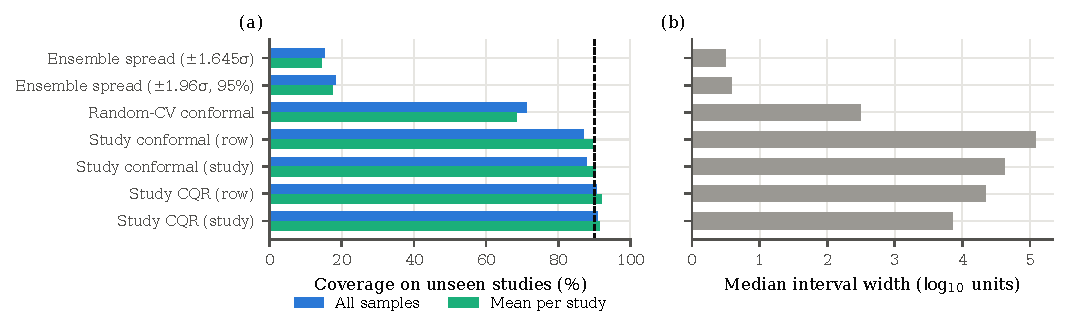
\includegraphics[width=\textwidth]{fig_intervals.pdf}
\caption{(a) Empirical coverage on unseen studies and (b) median interval width for baseline LightGBM, averaged over ten study-grouped fold assignments. The dashed line marks the 90\% target.}
\label{fig:intervals}
\end{figure*}

\subsection{Reliability Flags and Selective Prediction}

Table~\ref{tab:flags} shows that protocol mismatch, not distance, marks the worst predictions. Samples with a method string not seen in training are off by more than a factor of 100 in 57.9\% of cases, against 6.8\% for the rest. Bulk-water and pump samples behave similarly. A mesh outside the training range is rare (3.3\%) and covers two different cases. About half of the flagged samples come from the one 0.505~mm net study, the coarsest mesh in the data, which is flagged in every assignment and predicted normally (MAE 0.94, 4.0\% above $100\times$). The other half are the 0.45~$\mu$m membranes of Barrows~\textit{et al.} and Dehm~\textit{et al.} when both fall in the test fold, and these fail badly (MAE 2.99, 82.9\% above $100\times$). Distance over 500~km to any training sample does not matter (MAE 1.055 against 1.047). Distance to a training sample of the same family does (1.52 against 0.87).

Fig.~\ref{fig:risk} shows error as risky predictions are deferred. For the baseline, ranking by CQR width or by flag count works best. Deferring the widest 10\% of CQR intervals lowers MAE from 1.048 to 0.880 and the share of errors above $100\times$ from 14.2\% to 8.4\%. Deferring 20\% gives 0.824 and 6.5\%. Ensemble spread lowers error slowest down to 80\% retention, and same-family distance stops helping below it. Within-Between Physics starts lower and stays lower. Deferring the samples with the widest 10\% of baseline CQR intervals lowers its MAE from 0.929 to 0.836, and its errors above $100\times$ from 7.4\% to 5.6\%.

\begin{table}[!t]
\centering
\caption{Label-free reliability flags for baseline LightGBM on unseen studies, pooled over ten study-grouped fold assignments.}
\label{tab:flags}
\setlength{\tabcolsep}{2pt}
\begin{tabular}{@{}lccccc@{}}
\toprule
Flag & Share & \multicolumn{2}{c}{MAE} & \multicolumn{2}{c}{$>100\times$}\\
\cmidrule(lr){3-4}\cmidrule(lr){5-6}
 & & Flagged & Not & Flagged & Not\\
\midrule
Unseen method string & 14.4\% & 2.34 & 0.83 & 57.9\% & 6.8\%\\
Bulk water or pump & 16.2\% & 2.16 & 0.83 & 52.4\% & 6.8\%\\
Mesh outside training range & 3.3\% & 2.01 & 1.01 & 45.1\% & 13.1\%\\
$>500$~km to any sample & 8.4\% & 1.05 & 1.05 & 15.1\% & 14.1\%\\
$>500$~km to same family & 27.5\% & 1.52 & 0.87 & 30.3\% & 8.1\%\\
Widest 25\% of CQR intervals & 25.0\% & 1.71 & 0.83 & 37.3\% & 6.5\%\\
\bottomrule
\end{tabular}
\end{table}

\begin{figure*}[!t]
\centering
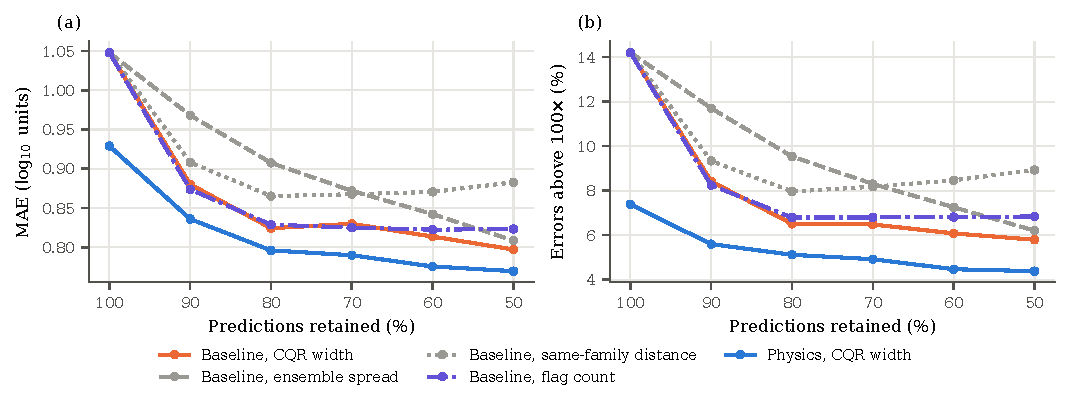
\includegraphics[width=\textwidth]{fig_risk_coverage.pdf}
\caption{(a) MAE and (b) share of errors above $100\times$ on retained unseen-study samples as the riskiest predictions are deferred, averaged over ten study-grouped fold assignments. Each curve pairs a model with a risk score.}
\label{fig:risk}
\end{figure*}

\subsection{Robustness of the Fixes}

Table~\ref{tab:robustness} repeats the main comparison on the reduced datasets. The constrained models beat the baseline on the full data, without the bongo-net study, and without Barrows and Dehm. With all three removed they lose (0.295 and 0.300 against 0.397) and beat the baseline in only 2 and 3 of 10 assignments. We had expected small leaves to explain this, since the reduced data leaves few bulk-water samples per leaf. Lowering the minimum leaf size from 30 to 10 changes nothing (0.297), so that explanation is wrong.

The cause is that the constrained models see only protocol features, and without the fine-mesh bulk-water studies protocol carries little that transfers. On this subset protocol-only LightGBM scores 0.263 by study and $-0.085$ by organization, and 91.7\% of the samples are surface nets. Two Sea Education Association studies with the same 0.335~mm mesh hold 56\% of the samples. Grouping by organization keeps them on the same side of every split, and every model drops: the baseline to 0.162, the constrained protocol model to 0.050, and Within-Between Physics to 0.075. The baseline keeps its lead because location and time, though weak alone (0.003 by organization), help it separate studies that protocol cannot. The constraints help on the data as archived, where bulk water and nets differ by orders of magnitude. Their gain depends on the bulk-water studies being present.

\begin{table}[!t]
\centering
\caption{Mean study-grouped \Rsq{} over ten fold assignments on reduced datasets, with the number of assignments won against the baseline in parentheses. Bold marks the best value in each row.}
\label{tab:robustness}
\setlength{\tabcolsep}{3pt}
\begin{tabular}{@{}lcccc@{}}
\toprule
Subset & Baseline & Constrained & Physics & Physics, leaf 10\\
\midrule
Full data & 0.456 & 0.543 (9) & \textbf{0.552} (10) & \textbf{0.552} (10)\\
Without bongo & 0.467 & 0.506 (8) & \textbf{0.507} (8) & 0.506 (8)\\
Without B\&D & 0.223 & 0.276 (6) & \textbf{0.294} (7) & 0.291 (7)\\
Without all three & \textbf{0.397} & 0.295 (2) & 0.300 (3) & 0.297 (3)\\
\bottomrule
\end{tabular}
\end{table}

\section{Discussion}

The results support four recommendations for anyone modeling pooled microplastic data.

\emph{Report study-grouped scores, averaged over fold assignments.} On NCEI data a random-split \Rsq{} mostly measures cruise recognition. A study-mean lookup scores 0.664 on random folds. A single study-grouped assignment can move \Rsq{} by more than 0.15, and pooled scores are dominated by the largest study, so a per-study error should sit beside them. Comparing MAE across papers also needs a common target scale, since $\log_{10}$, $\ln(c+1)$, and raw counts over a single basin give errors that cannot be compared directly.

\emph{Model protocol, and constrain it.} Mesh size, depth, and sampler family carry the cross-study signal. Shallow trees supply most of the gain, and a Huber loss with a monotonic mesh constraint cuts the largest errors further. They need no extra data and train faster than the unconstrained baseline. The gain depends on the bulk-water studies, so it should be checked again on any corrected or extended version of the archive.

\emph{Keep place-based terms out of the between-study offset, and treat zeros as censored.} Place descriptors fitted to raw $y$ act as cruise proxies. A drift-accumulation field fitted only to within-study variation helps a little on the global score and clearly inside surface-net studies, but its global effect is 0.009 and it adds nothing on the $\ln(c+1)$ scale. We do not present it as a new physical model. Modeling detection and the level of detected samples separately gives the best likelihood and shows that detected concentrations are far more predictable across studies than the pooled score suggests. A Tobit model ranks detections better but is worse calibrated.

\emph{Calibrate across studies and defer out-of-support cases.} Ensemble spread covers under 20\% of unseen-study samples at a nominal 90\%. Study-grouped CQR gives nominal coverage, and flags based on the sampling method catch most of the worst errors.

\subsection{Limitations}

Each survey usually uses one protocol in one region, so observational data cannot fully separate the selectivity of the sampler from unrecorded laboratory practice or from sampled volume, which drives zero counts. The drift field uses annual-mean velocities, and wind-driven vertical mixing at the sampling date is untested. All validation stays inside NCEI. AOMI~\cite{isobe2021} cannot serve as an independent test because it draws several of the same surveys from NCEI, so a clean non-NCEI test set remains future work. The bongo-net values stay unverified, and the Dehm correction rests on the abstract. Finally, we designed each fix after inspecting out-of-fold error on the same 72 studies, so the reported gains may partly reflect overfitting to these studies.

\section{Conclusion}

On 16,988 ocean-water samples from 72 NCEI studies, random cross-validation overstates the accuracy of predictions for a new study by about 0.31 in \Rsq{}. Location and time transfer nothing to unseen studies, and sampling protocol carries what does transfer, much of it through two bulk-water studies with corrected units. Shallow trees with a Huber loss and a monotonic mesh constraint raise the ten-assignment mean \Rsq{} from 0.456 to 0.543 and halve errors larger than a factor of 100, though weighted per study the error barely moves. A within-study drift term adds a small, consistent gain (0.552). A two-part model gives the best likelihood and reaches \Rsq{}~=~0.815 on detected samples. Study-grouped CQR gives 90.9\% coverage where ensemble spread gives 15.2\%. The constrained models lose their advantage when the disputed studies are removed. Predicting zeros, future surveys, and new organizations' net surveys is still unsolved. The next step is a test on observations from outside NCEI.

\section*{Data and Code Availability}

All code, the NCEI export, the unit corrections, and the drifter field are available at \url{https://github.com/zytact/marine-microplastics}. The script \texttt{experiments.py} reproduces Tables~\ref{tab:baseline}, \ref{tab:sensitivity}, \ref{tab:intervals}, and~\ref{tab:flags}, and the environmental-covariate, calibration, and ranking results. The script \texttt{experiments\_v2.py} reproduces the remaining tables, and \texttt{paper/figures.py} draws the figures from their output.

\bibliographystyle{IEEEtran}
\bibliography{references}

\end{document}
